\documentclass[runningheads]{llncs}
\usepackage[utf8]{inputenc}
\usepackage{float}
\usepackage{amsmath}
%\usepackage{amsthm}
\usepackage[colorlinks,citecolor=blue,linkcolor=blue,bookmarks=false,hypertexnames=true]{hyperref}
\usepackage{algorithm}
\usepackage{algpseudocode}
\usepackage{graphicx}
\usepackage{rotating,booktabs,multirow}
\usepackage[section]{placeins}
\usepackage[euler]{textgreek}
\usepackage[T1]{fontenc}

%misc libraries goes here
\usepackage{tikz}
\usetikzlibrary{automata,positioning}

\begin{document}

\title{Using Genetic Algorithms to Construct Slowly Synchronizing Finite State Machines}
\titlerunning{Genetic Algorithms to Construct Slowly Synchronizing FSMs}

\author{Adnan Kaan Ekiz  \and Yi\u{g}it Aras Tunal{\i} \and
\c{S}eyma Selcan Ma\u{g}ara \and Berk \c{C}iri\c{s}ci \and Kamer Kaya \and H\"{u}sn\"{u} Yenig\"{u}n}
\authorrunning{A. K. Ekiz et al.}


\institute{Sabanci University, Faculty of Engineering and Natural Sciences, Istanbul, Turkey}
\maketitle

\begin{abstract}
Computation of a shortest synchronizing sequence of an automaton is an NP-Hard problem.The longest possible shortest path and it's structure is well known and studied. There are various automata having shorter synchronizing length than the maximum but still are considered slowly synchronizing finite state machines. They can be utilized in many ways, such as testing the performance of algorithms for the synchronizing sequences. In this paper we will use a Genetic Algorithm approach to generate slowly synchronizing finite state machines of different sizes.
\keywords{Finite State Machines \and Synchronizing Sequences \and Genetic Algorithms|}
\end{abstract}

\section{Introduction}
The synchronizing (or reset) sequence of an automaton is a specific sequence of inputs that brings all states of deterministic finite automaton to a particular state regardless of the initial state of the system. A DFA is called \textit{synchronizing} if it has a reset word and the minimum length of the synchronizing sequence is called \textit{reset length} or \textit{shortest synchronizing sequence length}.\par
In 1964, Cerný \cite{cerny} conjunctured that maximum length of the shortest synchronizing sequence is (n-1)\textsuperscript{2} for a DFA with n states. Automata with reset lengths close to the Černý bound, called extremal or slowly synchronizing, usually have many interesting properties \cite{podolak_roman_szykula_zielinski_2017}. However, there are a few known extremal automata  \cite{Ananichev_Gusev_Volkov_2010}.

\par If every state of an automaton can be reached from every other state following the directions of the edges, this automaton is called \textit{strongly connected}. An automaton is \textit{weakly connected} if there exist an undirected path between every pair of distinct states. An automaton should be at least weakly connected in order to have a synchronizing sequence. In this work, we have worked with strongly connected automatons unless stated otherwise. \par In this paper, genetic algorithms are used to generate slowly synchronizing (or hard) finite state machines from a set of randomly generated DFAs with short reset length.

\section{Preliminaries}
\par A Deterministic Finite Automaton is a tuple $A = (Q,\delta, \Sigma, q_{0}, F)$ where Q is a finite set of states, Σ is finite input alphabet,  $q_{0}$ is the initial state $ q_{0} \in Q $ and F is the final state set $F \subseteq Q $. δ
is the transition function (full function) where $\delta: Q \times \Sigma \rightarrow Q ; (q,\sigma) \rightarrow \delta (q,\sigma) \in Q  $. Visualization of an automaton as a graph is given in Figure~\ref{fig:A0}.

\begin{figure}[ht]
	\centering
		\centering
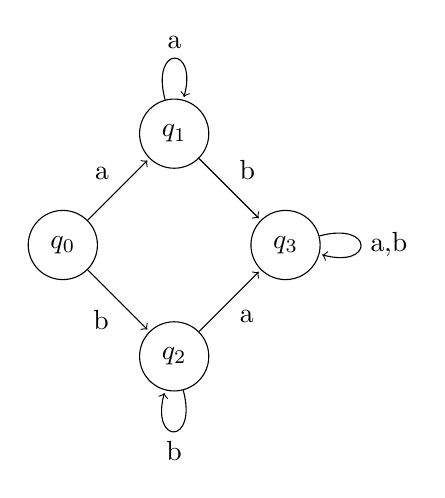
\begin{tikzpicture}[shorten >=1pt,node distance=2cm,on grid,auto]
   \node[state] (q_0)   {$q_0$};
   \node[state] (q_1) [above right=of q_0] {$q_1$};
   \node[state] (q_2) [below right=of q_0] {$q_2$};
   \node[state](q_3) [below right=of q_1] {$q_3$};
    \path[->]
    (q_0) edge  node {a} (q_1)
          edge  node [swap] {b} (q_2)
    (q_1) edge  node  {b} (q_3)
          edge [loop above] node {a} ()
    (q_3) edge [loop right] node {a,b} ()
    (q_2) edge  node [swap] {a} (q_3)
          edge [loop below] node {b} ();
\end{tikzpicture}
\caption{An automaton $A_1$}\label{fig:A0}
\end{figure}
\par A Deterministic Finite State Machine is a tuple $M = (Q,\delta, \Sigma, X, q_{0}, F)$ where Q is a finite set of states, $\Sigma$ is finite input alphabet,  $q_{0}$ is the initial state $ q_{0} \in Q $ and F is the final state set $F \subseteq Q $. $\delta$
is the transition function (full function) where $\delta: Q \times \Sigma \rightarrow (Q, x) ; (q,\sigma) \rightarrow \delta (q,\sigma) \in Q  $ The main difference of FSM from DFA is output symbols.In every transaction, an output symbol $x \in X$ is produced. Since output symbols are not taken into consideration while finding shortest synchronizing sequences, finite state machines are treated as DFAs.

\par An element $w \in \Sigma \textsuperscript{*}$ is called input sequence. Input sequence can be empty in this case denoted the length of the sequence $|w|$ is denoted as zero. Standard transition function returns the output for a single input letter therefore extended transition function, denoted by $\hat{\delta}$, is used for input sequences with $|w| > 1$. As the basis for extension  $\hat{\delta} (q, \epsilon) = q$. If input sequence $w$ is a word of the form $xa$ then $\hat{\delta} (q, w) = \delta(\hat{\delta}(q, x), a)$. In other words extended transition function returns the final state by recursively processing input word w.

\begin{definition}
For an automaton $A = (Q,\delta, \Sigma, q_{0}, F),$ a {\em Synchronizing Sequence (SS)} of $A$ is an input sequence $\bar{w}\in \Sigma^\star$ such that $|\hat{\delta}(Q,\bar{w})| = 1$.
\end{definition}

For instance, for the automaton $A_{1}$ given in Figure~\ref{fig:A0} and input sequence $w = ab$ all transitions end up with $q_{3}$ state no matter what the initial state is.

\par An FSM does not necessarily have a synchronizing sequence however existence of synchronizing sequence in an FSM is highly probable. Probability of having synchronizing sequence of an random FSM is $1-O(1/|Q|^{|\Sigma|})$
\cite{berlinkov}. Considering this high possibility, we randomly created sets of automatons and eliminated the ones without synchronizing sequence to constitute synchronizable automaton population. Existence check is polynomially bounded, there is an algorithm with complexity $O(|\Sigma||Q|^2)$ \cite{eppstein_1990} thus constructing an synchronizable automaton is quite fast. Another major problem with SS is finding the shortest synchronizable sequences.  Even though constructing a shortest synchronizing sequence is NP-hard problem, there are well studied heuristics algorithms to find a short SS. Eppstein showed that a short SS can be found using a greedy heuristic in time bounded by $O(n^3 + pn^2)$ where n is the number of states and p is the alphabet size\cite{eppstein_1990}.

\begin{figure}[ht]
		\centering
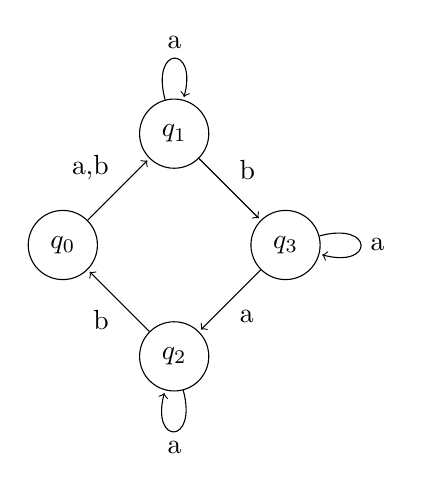
\begin{tikzpicture}[shorten >=1pt,node distance=2cm,on grid,auto]
   \node[state] (q_0)   {$q_0$};
   \node[state] (q_1) [above right=of q_0] {$q_1$};
   \node[state] (q_2) [below right=of q_0] {$q_2$};
   \node[state](q_3) [below right=of q_1] {$q_3$};
    \path[->]
    (q_0) edge  node {a,b} (q_1)
    (q_1) edge  node  {b} (q_3)
          edge [loop above] node {a} ()
    (q_3) edge [loop right] node {a} ()
          edge node {a} (q_2)
    (q_2) edge [loop below] node {a} (q_3)
          edge node {b} (q_0);
\end{tikzpicture}
\caption{An automaton which has $(n-1)^2$ length reset sequence (Cerný Conjecture)  $A_2$}\label{fig:A0}
\end{figure}

\newpage
\bibliographystyle{splncs04}
\bibliography{biby}
\end{document}
